\section{BPR}

\newcommand{\inputtextplus}[1][]{\ensuremath{\mathsf{T^{+}}\ifthenelse{\equal{#1}{}}{}{[#1]}}\xspace}
\newcommand{\rank}{\textit{rank}\xspace}
\newcommand{\coded}{\textit{code\textsubscript{d}}\xspace}
\newcommand{\bkt}{\textit{bkt}\xspace}
\newcommand{\offset}{\textit{offset}\xspace}
\newcommand{\covfefefe}{\texttt{covfefefe}\xspace}
\newcommand{\ovfefefe}{\texttt{ovfefefe}\xspace}
\newcommand{\vfefefe}{\texttt{vfefefe}\xspace}
\newcommand{\fefefe}{\texttt{fefefe}\xspace}
\newcommand{\efefe}{\texttt{efefe}\xspace}
\newcommand{\fefe}{\texttt{fefe}\xspace}
\newcommand{\efe}{\texttt{efe}\xspace}
\newcommand{\fe}{\texttt{fe}\xspace}
\newcommand{\e}{\texttt{e}\xspace}
\renewcommand{\O}{\mathcal{O}}


Der \currentauthor{Florian Grieskamp} im Jahr 2005 vorgestellte Algorithmus \bpr \cite{saca:2} erreicht trotz nicht optimaler asymptotischer Laufzeitschranke sehr schnelle Konstruktionszeiten von Suffixarrays für eine Vielzahl verschiedenartiger Strings. Aufgrund der daraus resultierenden Relevanz im Bereich der Textindexierung wird dieser Algorithmus hier im Rahmen der Projektgruppe \sacabench anhand einfacher Beispiele aufgearbeitet, wobei neben der Funktionsweise auch Laufzeit und Speicherbedarf im Vordergrund stehen.\par
Die Ziele des \bpr-Algorithmus von Schürmann und Stoye sind eine weniger komplexe Verarbeitung im Vergleich zu anderen Algorithmen sowie gute praktische Laufzeiten. Dieser Algorithmus wird hier daher zunächst anhand eines geeigneten Beispiels erklärt und anschließend im Bezug auf Komplexität hinsichtlich Speicherbedarf und Laufzeit analysiert.

\subsection{Vorüberlegungen}
\label{bpr:vorueberlegungen}

Damit einige der Schritte im späteren Verlauf des Algorithmus im Bezug auf Indizes außerhalb des zu verarbeitenden Strings wohldefiniert sind, betrachten wir häufig eine erweiterte Version eines Strings gemäß Definition \ref{def:tplus}. Abbildung \ref{fig:tplus} zeigt beispielhaft eine Erweiterung eines Strings.

\begin{figure}[ht]
	\resizebox{\textwidth}{!}{
		\begin{tabular}{@{}l@{}}
			\includegraphics{kapitel/saca_algorithmen/bpr/algorithmus/phase1/t/image.pdf} \\
			\includegraphics{kapitel/saca_algorithmen/bpr/algorithmus/phase1/tplus/image.pdf}
		\end{tabular}
	}
	\caption{Erweiterung von \inputtext zu \inputtextplus durch Anhängen von \(\$^n\)}
	\label{fig:tplus}
\end{figure}

\begin{definition}[\inputtextplus]
	\label{def:tplus}
    Sei \(\Sigma\) ein total geordnetes endliches Alphabet und \(\inputtext = \inputtext[0] \inputtext[1] \ldots \inputtext[n-1] \in \Sigma\) ein String über \(\Sigma\). Sei außerdem \(\$ \notin \Sigma\) ein nicht in \(\Sigma\) enthaltenes Symbol mit \(\forall c \in \Sigma : \$ < c\). Den um \(\$^n\) erweiterten String \(\inputtext\$^n\) nennen wir \inputtextplus.
\end{definition}

Ist das zugrunde liegende Alphabet außerdem total geordnet, so können auch die Suffixe eines Strings anhand dieser Ordnung sortiert werden.
Der Vergleich zweier Symbole des Alphabets bezüglich der Ordnung wird dadurch vereinfacht, dass jedem Symbol mit der Funktion \effective (Definition \ref{def:effective_alphabet} auf Seite \pageref{def:effective_alphabet}) eine natürliche Zahl als Rang zugewiesen wird.

Während für einzelne Symbole die Verwendung des effektiven Alphabets gegenüber dem direkten Vergleich keinen wesentlichen Vorteil erzielt, ergibt sich bei dem lexikographischen Vergleich zweier Strings bereits eine andere Situation: Auf Basis der Ränge der einzelnen Symbole kann auch ganzen Strings eine ganzzahlige Codierung zugewiesen werden, welche den Vergleich beschleunigt.

\begin{definition}[Stringkodierung]
	\label{def:coded}
	Sei \(\coded : (\Sigma \cup \{\$\})^d \rightarrow \{0, \ldots, (|\Sigma| + 1)^d - 1\}\) eine bijektive Funktion\footref{differs_from_paper}, sodass für zwei Strings \(u, v \in (\Sigma \cup \{\$\})^d\) gilt \(u < v \Leftrightarrow \coded(u) < \coded(v)\).
\end{definition}

Eine Stringkodierung wie in Definition \ref{def:coded} kann einfach unter Verwendung einer gegebenen \effective-Funktion (Definition \ref{def:effective_alphabet}) realisiert werden, indem die Symbole eines Strings abhängig von ihrem Index mit absteigender Wertigkeit für höhere Indizes summiert werden. Auf diese Weise ergibt sich für einen String \(\inputtext{[i,i+d)} = \inputtext[i] \ldots \inputtext[i + d - 1]\) die Kodierung \[\coded(\inputtext{[i,i+d)}) = \sum_{j=0}^{d - 1} (|\Sigma| + 1)^{d - 1 - j} \cdot \effective(\inputtext[i + j]).\]\par\smallskip
Auch Kodierungen für Strings größerer Länge als \(d\) können auf diese Weise berechnet werden, indem alle Symbole an Indizes größer oder gleich \(d\) ignoriert werden. Aufgrund der hier gewählten Berechnungsvorschrift für \coded lassen sich außerdem auf sehr einfache Weise Kodierungen für aufeinanderfolgende Suffixe berechnen.
\begin{equation}
	\label{eq:coded}
    \coded(\suffix{i+1}) = (|\Sigma| + 1) \cdot \left( \coded(\suffix{i}) \text{ mod } (|\Sigma| + 1)^{d-1}\right) + \effective(\inputtextplus[i+d])
\end{equation}
Man beachte hier, dass für zwei aufeinanderfolgende Suffixe \suffix{i} und \suffix{i+1} lediglich das erste Symbol aus \suffix{i} aus der Kodierung entfernt werden muss (mittels mod \((|\Sigma| + 1)^{d-1}\)), woraufhin die Wertigkeit aller verbleibenden Symbole jeweils um eine Stelle ansteigt. Zuletzt muss nur noch der Rang des letzten Symbols aus \suffix{i+1} hinzu addiert werden.\par\smallskip
Wie viele andere Algorithmen zur Konstruktion von Suffixarrays, arbeitet auch \bpr mit einer Unterteilung des Suffixarrays in sogenannte Buckets (Definition \ref{def:bucket} auf Seite \pageref{def:bucket}). Die Unterteilung des Arrays in Buckets ist erforderlich, um das Suffixarray schrittweise sortieren zu können, indem bestehende Buckets durch Aufteilung weiter verfeinert werden.

\subsection{Algorithmus}
\label{bpr:algorithmus}

Nachdem in Kapitel \ref{bpr:vorueberlegungen} bereits die formalen Grundlagen für die Beschreibung des \bpr-Algorithmus geschaffen wurden, können wir nun präziser auf die Funktionsweise des Algorithmus eingehen. Die Basis für das Verfahren bildet die Nutzung von Abhängigkeiten zwischen mehreren Suffixen: Teilen sich zwei Suffixe \suffix{i} und \suffix{j} einen gemeinsamen Präfix der Länge \(\textit{offset}\), so ist zunächst festzustellen, dass \suffix{i+\textit{offset}} bzw. \suffix{j+\textit{offset}} nicht nur Suffixe von \inputtext, sondern auch Suffixe von \suffix{i} bzw. \suffix{j}  sind. Die Reihenfolge von \suffix{i} und \suffix{j} im Suffix-Array kann also einfach durch die Reihenfolge der eventuell bereits zuvor sortierten Suffixe \suffix{i+\textit{offset}} und \suffix{j+\textit{offset}} bestimmt werden. Um allerdings auf eine derartige Vorsortierung zurückgreifen zu können, muss zu Beginn zumindest eine grobe \glqq initiale Sortierung\grqq{} der Suffixe existieren.\par\smallskip
Um dies zu erreichen, verwendet der hier beschriebene Algorithmus zwei Phasen, von denen die erste dazu dient, die Suffixe initial nach gemeinsamen Präfixen der Länge \(d\) zu gruppieren. Auf Basis dieser Gruppierung werden die Suffixe Buckets zugewiesen, sodass sich zwei Suffixe genau dann im gleichen Bucket befinden, wenn sie einen gemeinsamen Präfix der Länge \(d\) besitzen.\par
In der zweiten Phase werden dann die Buckets anhand der oben genannten Vorschrift schrittweise rekursiv verfeinert. Auf diese Weise ergibt sich das fertig sortierte Suffix-Array, sobald jeder Bucket eine minimale Länge von 1 erreicht hat.\par\smallskip
Im Folgenden werden beide Phasen im Detail erklärt. Wir verwenden dafür als Beispiel das Fantasiewort \covfefefe, dessen Suffixe wir mittels \bpr sortieren.

\subsubsection{Erste Phase}
\label{bpr:algorithmus:phase1}

Die erste Phase führt eine Gruppierung der Suffixe nach gemeinsamen Präfixen der Länge \(d\) durch. Die Wahl eines geeigneten Parameters \(d\) wird nicht vom Algorithmus übernommen, es wird allerdings empfohlen, \(d < \log n\) zu wählen \cite{saca:2}.\par
Um nun alle Suffixe von \inputtext in Level-\(d\)-Buckets zu gruppieren, wird zunächst eine Tabelle \bkt der Länge \((|\Sigma| + 1)^d\) mit Einträgen für alle möglichen Präfixe der Länge \(d\) erstellt, wobei jeder Präfix eindeutig durch den zugehörigen Funktionswert von \coded identifiziert werden kann. In einem sequentiellen Durchlauf des Textes \inputtextplus können dann mithilfe der Eigenschaft aus Gleichung \ref{eq:coded} die Kodierungen der vorkommenden Präfixe effizient berechnet werden. In diesem Durchlauf kann für jeden Präfix \(p\) die zugehörige Anzahl der Vorkommen in \inputtextplus (und damit die spätere Größe des Buckets \(b_p\)) bestimmt werden.\par
Da die Sortierung der Buckets durch den Schlüssel \coded gegeben ist, können im Anschluss anhand der nun bekannten Bucketgrößen auch die Positionen aller Buckets im Suffixarray festgelegt werden.
\begin{figure}[ht]
	\vspace{0.2\baselineskip}
	\resizebox{\textwidth}{!}{
		\includegraphics{kapitel/saca_algorithmen/bpr/algorithmus/phase1/bkt/image.pdf}
	}
	\caption[Tabelle \emph{bkt} zur Bestimmung der Bucket-Größen und -Positionen]{Tabelle \emph{bkt} zur Bestimmung der Bucket-Größen und -Positionen. Die Anzahl der Vorkommen eines Präfix im Text ist in Zeile 2 angegeben. Zeile 3 beinhaltet die kumulierte Anzahl und bestimmt damit die linke Grenze des nachfolgenden Buckets.}
	\label{fig:bkt}
\end{figure}
Der entsprechende Stand der Verarbeitung für den Text \(\inputtext = \covfefefe\) ist in Abbildung \ref{fig:bkt} zu sehen. Die kumulierte Größe aller Buckets bis einschließlich Bucket \(j\) legt gleichzeitig die linke Grenze des Buckets \(j+1\) fest. In einem weiteren Durchlauf können jetzt alle Suffixe \(\suffix{0}, \ldots, \suffix{n-1}\) im vorläufigen Suffixarray \sa einsortiert werden. Das Suffixarray beinhaltet dabei für ein Suffix \suffix{i} mit \(0 \leq i < n\) nicht das gesamte Suffix als String, sondern lediglich den Index \(i\) des Suffixes. Abbildung \ref{fig:buckets_initial} zeigt die initiale Einteilung der Buckets für \(d=2\). Zur besseren Visualisierung sind hier in dem Array die Suffixe anstatt der bloßen Indizes angegeben.\par\smallskip
\begin{figure}[ht]
	\resizebox{\textwidth}{!}{
		\includegraphics{kapitel/saca_algorithmen/bpr/algorithmus/phase1/sa_initial/image.pdf}
		\hspace{1em}
		\includegraphics{kapitel/saca_algorithmen/bpr/algorithmus/phase1/buckets_initial/image.pdf}
	}
	\caption[Suffixe unsortiert und nach der ersten Phase des Algorithmus]{Suffixe unsortiert (links) und nach der ersten Phase des Algorithmus (rechts)}
	\label{fig:buckets_initial}
\end{figure}
Wie bereits zuvor erwähnt, wollen wir in der zweiten Phase des Algorithmus die Buckets verfeinern, indem eine weitere Gruppierung jedes bestehenden Buckets aufgebaut wird.\par
\begin{wrapfigure}[15]{r}{0.42\textwidth}
	\vspace{-1em}
	\resizebox{0.42\textwidth}{!}{
		\includegraphics{kapitel/saca_algorithmen/bpr/algorithmus/phase1/buckets_initial_plain/image.pdf}
	}\\
	\resizebox{0.42\textwidth}{!}{
		\includegraphics{kapitel/saca_algorithmen/bpr/algorithmus/phase1/bptr_initial/image.pdf}
	}
	\caption[Vorsortierte Suffixe und zugehörige Bucket-Pointer]{Vorsortierte Suffixe und zugehörige Bucket-Pointer}
	\label{fig:bucket_pointer_initial}
\end{wrapfigure}
Wir wollen dazu auf die bereits bekannte Einteilung der Suffixe in Level-\(d\)-Buckets zugreifen und anhand dessen eine weiterführende Sortierung vollziehen. Eine Anfrage, in welchem Bucket sich ein Suffix befindet, ist jedoch mit der bisher eingeführten Datenstruktur nicht effizient zu beantworten. \par
Es wird daher mit dem Bucket Pointer \bptr ein zweites Array eingeführt, welches sinngemäß ein Reverse Mapping des Suffixarrays \sa beinhaltet (s. Abbildung \ref{fig:bucket_pointer_initial}). In diesem Array symbolisiert jeder Index ein Suffix, wobei der Eintrag \(\bptr[i]\) den zugehörigen Bucket angibt, welcher jeweils über seine rechte Grenze identifiziert wird. Die Bestimmung der Grenzen erfolgt durch Ablesen der kumulierten Summe aus der Tabelle \bkt.

\subsubsection{Zweite Phase}
\label{bpr:algorithmus:phase2}

Zu Beginn dieser Phase des Algorithmus existiert bereits ein (noch nicht fertig sortiertes) Suffixarray \sa, welches nun rekursiv sortiert werden soll. Die aktuelle Einteilung der Suffixe in Buckets ist über den Bucket Pointer \bptr gegeben, aus dem abgelesen werden kann, ob sich zwei Suffixe im gleichen oder in verschiedenen Buckets befinden. Das Array \bkt, welches in der ersten Phase des Algorithmus erstellt wurde, um die initiale Zuteilung festzulegen, wird im weiteren Verlauf nicht mehr verwendet.\par
Die Sortierung erfolgt rekursiv für jeden Bucket im Suffixarray. Da die einzelnen Buckets untereinander zu jedem Zeitpunkt bereits sortiert sind, muss der Sortiervorgang in jedem Rekursionsschritt nur innerhalb des jeweiligen Buckets stattfinden. Da es für effizientes Sortieren aber erforderlich ist, zwei Suffixe mit konstantem Aufwand vergleichen zu können, werden wir zunächst sehen, anhand welcher Kriterien wir Suffixe effizient vergleichen können.
\begin{figure}[ht]
	\resizebox{\textwidth}{!}{
			\includegraphics{kapitel/saca_algorithmen/bpr/algorithmus/phase2/buckets_initial_compare/image.pdf}
			\hspace{1em}
			\includegraphics{kapitel/saca_algorithmen/bpr/algorithmus/phase2/buckets_initial_compare_highlight/image.pdf}
	}
	\caption{Vergleich zweier Suffixe innerhalb eines Buckets}
	\label{fig:inner_bucket}
\end{figure}
Am bereits zuvor eingeführten Beispiel beginnen wir, den Bucket \bucket{\textup{ef}} zu sortieren (Abbildung~\ref{fig:inner_bucket}). Der Bucket beinhaltet die Suffixe \suffix{4} und \suffix{6}, welche nach dem Sortierschritt in Phase 1 einen gemeinsamen Präfix der Länge \(d = 2\) haben. Da die Sortierung der Suffixe lexikographisch erfolgen soll, können gemeinsame Präfixe ignoriert werden, ohne die Korrektheit der Sortierung zu beeinflussen. 
\begin{lemma}[Gemeinsamer Präfix]
	\label{lemma:common_prefix}
	\normalfont
    Haben zwei Suffixe \suffix{i} und \suffix{j} einen gemeinsamen Präfix der Länge \offset, so ist \(\suffix{i} \leq \suffix{j}\) genau dann, wenn \(\suffix{i+\offset} \leq \suffix{j+\offset}\). Dies folgt direkt aus der Definition der lexikographischen Ordnung.
\end{lemma}
Für Suffixe \(\suffix{i}, \suffix{j}\) mit \(i, j \in \mathsf{b}\) gibt der Level des Buckets \(\mathsf{b}\) eine untere Schranke für \offset an. Im Falle des Beispiels genügt es also, die Suffixe \(\suffix{4+2} = \suffix{6}\) und \(\suffix{6+2} = \suffix{8}\) zu vergleichen (Abbildung~\ref{fig:buckets_compare_and_sort}, oben links). Da selbstverständlich Suffixe der Suffixe von \inputtext auch selbst Suffixe von \inputtext sind, befinden sich auch diese in \sa. Falls  sich \(\suffix{i+\offset}\) und \(\suffix{j+\offset}\) bereits in verschiedenen Buckets befinden, ist das lexikographische Verhältnis dieser beiden Suffixe bereits bekannt. Um dies herauszufinden, werden die Bucket Pointer der entsprechenden Suffixe verglichen. Diese befinden sich im Array \bptr, welches bereits in Phase 1 initialisiert wurde und beinhalten einen Verweis auf die rechte Grenze des Buckets, in dem sich der jeweilige Suffix befindet.\par
\begin{figure}[ht]
	\resizebox{\textwidth}{!}{
		\includegraphics[valign=t]{kapitel/saca_algorithmen/bpr/algorithmus/phase2/buckets_initial_compare_highlight_label/image.pdf}
		\hspace{1em}
		\includegraphics[valign=t]{kapitel/saca_algorithmen/bpr/algorithmus/phase2/buckets_updated/image.pdf}
	}\vspace{1ex}
	\resizebox{\textwidth}{!}{
		\includegraphics[valign=t]{kapitel/saca_algorithmen/bpr/algorithmus/phase2/bptr_initial_highlighted/image.pdf}
		\hspace{1em}
		\includegraphics[valign=t]{kapitel/saca_algorithmen/bpr/algorithmus/phase2/bptr_updated/image.pdf}
	}
	\caption[Buckets sowie Bucket-Pointer vor und nach der ersten Verfeinerung]{Buckets (oben) sowie Bucket-Pointer (unten) vor und nach der ersten Verfeinerung. Es ist gut zu erkennen, dass bereits bei einer Rekursionstiefe von 1 nur noch ein nicht eindeutig sortierter Bucket existiert.}
	\label{fig:buckets_compare_and_sort}
\end{figure}
Abbildung~\ref{fig:buckets_compare_and_sort} (unten links) zeigt die Bucket Pointer der Suffixe \(\suffix{6}\) (Bucket \(\bucket{\textup{ef}}\) mit rechter Grenze an Index 3 in \sa) und \(\suffix{8}\) (Bucket \(\bucket{\textup{e\$}}\) mit rechter Grenze an Index 1 in \sa). Aus einem einfachen Vergleich dieser Bucket Pointer geht hervor, dass \(\suffix{8}\) lexikographisch kleiner ist als \(\suffix{6}\). Mithilfe von Lemma \ref{lemma:common_prefix} kann daraus geschlossen werden, dass auch \(\suffix{6}\) lexikographisch kleiner ist als \(\suffix{4}\). Ein solcher Vergleich kann durch zwei Zugriffe auf das Array \bptr in konstanter Zeit durchgeführt werden. Zur Veranschaulichung zeigt Abbildung~\ref{fig:buckets_compare_and_sort} (rechts) den Zustand von \sa und \bptr, wenn in \sa nur noch Level-4-Buckets enthalten sind. Nachdem ein Verfeinerungsschritt in einem Bucket \(\bucket{\textup{p}} = [l,r]\) in kleinere Buckets durchgeführt wurde, müssen außerdem die zugehörigen Bucket-Pointer im Array \bptr angepasst werden. Dazu wird der Bucket \(\bucket{\textup{p}}\) von rechts nach links durchlaufen, wobei für jeden darin enthaltenen Suffix \(\sa[i], l \leq i \leq r,\) der Sortiertschlüssel \(\bptr[\sa[i]+\offset]\) abgefragt. Es wird dann zwischen zwei Fällen unterschieden:

\begin{description}
	\item[Fall 1:]\(\bptr[\sa[i-1]+\offset] = \bptr[\sa[i]+\offset]\) \\
		Die Sortierschlüssel der Suffixe \(\sa[i-1]\) und \(\sa[i]\) sind identisch. Daher konnte in diesem Schritt keine echte Sortierung dieser beiden Suffixe vorgenommen werden. Deshalb befinden sie sich nach wie vor in einem gemeinsamen Bucket und \(\bptr[\sa[i-1]]\) wird auf \(\bptr[\sa[i]]\) gesetzt.
	\item[Fall 2:] \(\bptr[\sa[i-1]+\offset] \neq \bptr[\sa[i]+\offset]\) \\
		Die Sortierschlüssel der Suffixe \(\sa[i-1]\) und \(\sa[i]\) unterscheiden sich. Die Suffixe konnten also sortiert werden und befinden sich nach der Verfeinerung in unterschiedlichen Buckets. \(\sa[i-1]\) ist das erste Element von rechts in dem neu beginnenden Bucket. Folglich wird \(\bptr[\sa[i-1]]\) auf \(i-1\) gesetzt.
\end{description}

\noindent Nachdem die Bucket-Pointer aktualisiert wurden, ist der Sortiervorgang für \(\bucket{\textup{p}}\) abgeschlossen und es kann rekursiv fortgefahren werden. Das fertig sortierte Suffixarray (links), welches nach Abschluss der Sortierung nur noch Buckets der Größe 1 enthält, sowie die dazugehörigen Bucket-Pointer (rechts) sind in Abbildung~\ref{fig:buckets_final} zu sehen.\par\smallskip
\begin{figure}[ht]
	\resizebox{\textwidth}{!}{
		\includegraphics{kapitel/saca_algorithmen/bpr/algorithmus/phase2/buckets_final/image.pdf}
		\hspace{1em}
		\includegraphics{kapitel/saca_algorithmen/bpr/algorithmus/phase2/bptr_final/image.pdf}
	}
	\caption[Sortiertes Suffix-Array und zugehörige Bucket-Pointer]{Sortiertes Suffix-Array (links) und zugehörige Bucket-Pointer (rechts)}
	\label{fig:buckets_final}
\end{figure}
Bei der Wahl des Sortierverfahrens unterscheidet \bpr abhängig von der Größe eines Buckets zwischen \emph{Insertionsort} und \emph{Quicksort}. Für Buckets mit maximal 15 Elementen wird \emph{Insertionsort} verwendet, während alle größeren Buckets mit einer Variante von \emph{Quicksort} sortiert werden. Ergänzend zur Partitionierung des Buckets in zwei Hälften werden alle an das Pivotelement angrenzenden Elemente mit gleichem Sortierschlüssel von den rekursiv zu sortierenden Partitionen ausgenommen, solange bis in beide Richtungen das erste Element mit unterschiedlichem Schlüssel gefunden wird. Diese Heuristik sorgt dafür, dass je nach Struktur des Eingabestrings die zu sortierenden Partitionen deutlich verkleinert werden können, falls in einem Bucket viele Suffixe den gleichen Schlüssel haben.\par\smallskip
Falls es aufgrund der Struktur des Eingabestrings vorkommt, dass innerhalb eines Buckets alle Suffixe einen gemeinsamen Präfix einer deutlich größeren Länge als \offset haben, dann würde \emph{Quicksort} (bzw. bei kleinen Buckets \emph{Insertionsort}) für mehrere Schritte in der Rekursion versuchen, ausschließlich Elemente mit gleichem Schlüssel zu sortierten. Dies beeinflusst zwar nicht die Korrektheit des Verfahrens, allerdings entsteht durch jeden überflüssigen Sortiervorgang ein unerwünschter und vermeidbarer Aufwand. Um dem entgegen zu wirken, wird eine Heuristik verwendet, welche nach einem \glqq erfolglosen\grqq{} Sortiervorgang die Länge des längsten gemeinsamen Präfixes aller Suffixe in diesem Bucket bestimmt. Der darauf folgende Rekursionsschritt wird dann mit dieser Länge anstelle von \offset aufgerufen.

\subsubsection{Beispiel}
\label{bpr:algorithmus:beispiel}

\newcolumntype{M}[1]{>{\centering\arraybackslash}m{#1}}
\newcommand{\mc}[2]{\multicolumn{#1}{c}{#2}}

Am Beispiel \texttt{caabaccaabacaa} wird noch einmal die Funktionsweise des gesamten Algorithmus im Detail demonstriert. Das Beispiel dient der Übersichtlichkeit und Vergleichbarkeit zu anderen Algorithmen.
\begin{figure}[ht]
    {\centering\begin{minipage}{\textwidth}
        {\large \textsc{Schritt 1}} \hfill {\Large \textsc{Phase 1}}\par\medskip
        \resizebox{\textwidth}{!}{\includegraphics{kapitel/saca_algorithmen/bpr/algorithmus/beispiel/phase_1/step_01/t/image.pdf}}\par\bigskip
        \resizebox{\textwidth}{!}{\includegraphics{kapitel/saca_algorithmen/bpr/algorithmus/beispiel/phase_1/step_01/tplus/image.pdf}}\\
    \end{minipage}}
    \caption[\bpr: Phase 1, Schritt 1]{\bpr: Phase 1, Schritt 1. Oben: Eingabetext \inputtext. Unten: Erweiterter Eingabetext \inputtextplus.}
    \label{bpr:p1s1}
\end{figure}
Der erste Schritt besteht lediglich daraus, die Eingabe aufzubereiten, indem \(n\) symbolische Sentinels an das Eingabewort angehängt werden. Dieses Vorgehen wird im Paper beschrieben, im Algorithmus allerdings aufgrund des linearen Speicherbedarfs nicht direkt umgesetzt. \par
\begin{figure}[ht]
    {\centering\begin{minipage}{\textwidth}
        {\large \textsc{Schritt 2}}\par\medskip
        \resizebox{\textwidth}{!}{\includegraphics{kapitel/saca_algorithmen/bpr/algorithmus/beispiel/phase_1/step_02/bkt/image.pdf}}\par\medskip
        \resizebox{\textwidth}{!}{\includegraphics{kapitel/saca_algorithmen/bpr/algorithmus/beispiel/phase_1/step_02/buckets/image.pdf}}
    \end{minipage}}
    \caption[\bpr: Phase 1, Schritt 2]{\bpr: Phase 1, Schritt 2. Oben: Größen und Positionen der Buckets. Unten: Leere Buckets im Suffix-Array.}
    \label{bpr:p1s2}
\end{figure}
Im zweiten Schritt wird der Bucketsort Algorithmus (\cref{section:bucketsort}) durchgeführt, um eine Vorsortierung für das Suffix-Array zu erlangen. Die Tiefe, die für Bucketsort als Parameter verwendet wird, leitet sich in festgelegten Stufen aus der Größe des Alphabets ab und beträgt auch für große Alphabete mindestens 3. In diesem Beispiel wird aus Gründen der Übersichtlichkeit nur eine Tiefe von 2 verwendet.\par
\begin{figure}[H]
    {\centering\begin{minipage}{\textwidth}
        {\large \textsc{Schritt 3}}\par\medskip
        \resizebox{\textwidth}{!}{
            \includegraphics{kapitel/saca_algorithmen/bpr/algorithmus/beispiel/phase_1/step_03/buckets/image.pdf}
        }
        \resizebox{\textwidth}{!}{
            \includegraphics{kapitel/saca_algorithmen/bpr/algorithmus/beispiel/phase_1/step_03/bptr/image.pdf}
        }
    \end{minipage}}
    \caption[\bpr: Phase 1, Schritt 3]{\bpr: Phase 1, Schritt 3. Links: Befüllte Buckets im Suffix-Array. Rechts Initiales \bptr-Array.}
    \label{bpr:p1s3}
\end{figure}
Zu Beginn des dritten Schrittes sind die rechten Grenzen der Buckets bereits bekannt (siehe \cref{bpr:p1s2}, rot markiert und \cref{bpr:p1s3}, oben) und die Suffixe in die entsprechenden Buckets einsortiert. Daraus wird im Anschluss das Bucket-Pointer Array (\cref{bpr:p1s3}, unten) berechnet, in dem für jeden Suffix gespeichert ist, in welchem Bucket sich dieser in der aktuellen Sortierung befindet. Die Buckets werden dabei über ihre rechte inklusive Grenze identifiziert.\par
Sobald die Bucket-Pointer bestimmt sind, ist ein Zustand erreicht, von dem aus im Anschluss in der zweiten Phase alle Buckets Schritt für Schritt verfeinert werden können. Diese Verfeinerung erfolgt iterativ über die Buckets und rekursiv innerhalb der Buckets. Die Reihenfolge, in der die nach Phase 1 entstandenen Buckets sortiert werden, ist im Grundalgorithmus für die Korrektheit irrelevant. Unter Verwendung der Copy-Technik lässt sich der Rechenaufwand aber durch eine geschickte Wahl der Reihenfolge verringern.\par
\begin{figure}[H]
    {\centering\begin{minipage}{\textwidth}
        {\large \textsc{Schritt 1 (vorher)}} \hfill {\Large \textsc{Phase 2}}\par\medskip
        \resizebox{\textwidth}{!}{\includegraphics{kapitel/saca_algorithmen/bpr/algorithmus/beispiel/phase_2/step_01/buckets_before/image.pdf}}
        \resizebox{\textwidth}{!}{\includegraphics{kapitel/saca_algorithmen/bpr/algorithmus/beispiel/phase_2/step_01/bptr_before/image.pdf}}
    \end{minipage}}
    \caption[\bpr: Phase 2, Schritt 1 (vorher)]{\bpr: Phase 2, Schritt 1. \sa und \bptr vor dem Sortierschritt.}
    \label{bpr:p2s1:1}
\end{figure}
\begin{figure}[H]
    {\centering\begin{minipage}{\textwidth}
        {\large \textsc{Schritt 1 (nachher)}} \hfill {\Large \textsc{Phase 2}}\par\medskip
        \resizebox{\textwidth}{!}{\includegraphics{kapitel/saca_algorithmen/bpr/algorithmus/beispiel/phase_2/step_01/buckets_after/image.pdf}}
        \resizebox{\textwidth}{!}{\includegraphics{kapitel/saca_algorithmen/bpr/algorithmus/beispiel/phase_2/step_01/bptr_after/image.pdf}}
    \end{minipage}}
    \caption[\bpr: Phase 2, Schritt 1 (nachher)]{\bpr: Phase 2, Schritt 1. \sa und \bptr nach dem Sortierschritt.}
    \label{bpr:p2s1:2}
\end{figure}
Die Verfeinerung erfolgt innerhalb eines Buckets Schrittweise mit einer Schrittgröße, die der zuvor gewählten Tiefe von Bucketsort entspricht. In diesem Beispiel wird zuerst der Bucket \bucket{ab} verfeinert. Aus der Bucket-Pointer Tabelle lässt sich nach einem Rekursionsschritt ablesen, dass die beiden darin enthaltenen Suffixe in ihrer Reihenfolge vertauscht werden müssen. Danach ist der Bucket fertig sortiert und die Bucket-Pointer werden an die neue Sortierung angepasst.\par
\begin{figure}[H]
    {\centering\begin{minipage}{\textwidth}
        {\large \textsc{Schritt 2 (vorher)}}\par\medskip
        \resizebox{\textwidth}{!}{\includegraphics{kapitel/saca_algorithmen/bpr/algorithmus/beispiel/phase_2/step_02/buckets_before/image.pdf}}
        \resizebox{\textwidth}{!}{\includegraphics{kapitel/saca_algorithmen/bpr/algorithmus/beispiel/phase_2/step_02/bptr_before/image.pdf}}
    \end{minipage}}
    \caption[\bpr: Phase 2, Schritt 2 (vorher)]{\bpr: Phase 2, Schritt 2. \sa und \bptr vor dem Sortierschritt.}
    \label{bpr:p2s2:1}
\end{figure}
\begin{figure}[H]
    {\centering\begin{minipage}{\textwidth}
        {\large \textsc{Schritt 2 (nachher)}}\par\medskip
        \resizebox{\textwidth}{!}{\includegraphics{kapitel/saca_algorithmen/bpr/algorithmus/beispiel/phase_2/step_02/buckets_after/image.pdf}}
        \resizebox{\textwidth}{!}{\includegraphics{kapitel/saca_algorithmen/bpr/algorithmus/beispiel/phase_2/step_02/bptr_after/image.pdf}}
    \end{minipage}}
    \caption[\bpr: Phase 2, Schritt 2 (nachher)]{\bpr: Phase 2, Schritt 2. \sa und \bptr nach dem Sortierschritt.}
    \label{bpr:p2s2:2}
\end{figure}
Anschließend wird der Bucket \bucket{ac} sortiert (\cref{bpr:p2s2:1,bpr:p2s2:2}), dessen Suffixe sich bereits nach einem gemeinsamen Präfix der Länge 2 unterscheiden. Aus der Bucket-Pointer Tabelle kann damit direkt abgelesen werden, in welchen Buckets sich die korrespondierenden Suffixe befinden, woraus dann die Reihenfolge abgeleitet wird. Das Vertauschen von \(\suffix{5}\) und \(\suffix{11}\) führt zur richtigen Reihenfolge.\par
Die darauf folgende Sortierung des Buckets \bucket{ba} erfolgt analog (\cref{bpr:p2s3:1,bpr:p2s3:2}).
\begin{figure}[H]
    {\centering\begin{minipage}{\textwidth}
        {\large \textsc{Schritt 3 (vorher)}}\par\medskip
        \resizebox{\textwidth}{!}{\includegraphics{kapitel/saca_algorithmen/bpr/algorithmus/beispiel/phase_2/step_03/buckets_before/image.pdf}}
        \resizebox{\textwidth}{!}{\includegraphics{kapitel/saca_algorithmen/bpr/algorithmus/beispiel/phase_2/step_03/bptr_before/image.pdf}}
    \end{minipage}}
    \caption[\bpr: Phase 2, Schritt 3 (vorher)]{\bpr: Phase 2, Schritt 3. \sa und \bptr vor dem Sortierschritt.}
    \label{bpr:p2s3:1}
\end{figure}
\begin{figure}[H]
    {\centering\begin{minipage}{\textwidth}
        {\large \textsc{Schritt 3 (nachher)}}\par\medskip
        \resizebox{\textwidth}{!}{\includegraphics{kapitel/saca_algorithmen/bpr/algorithmus/beispiel/phase_2/step_03/buckets_after/image.pdf}}
        \resizebox{\textwidth}{!}{\includegraphics{kapitel/saca_algorithmen/bpr/algorithmus/beispiel/phase_2/step_03/bptr_after/image.pdf}}
    \end{minipage}}
    \caption[\bpr: Phase 2, Schritt 3 (nachher)]{\bpr: Phase 2, Schritt 3. \sa und \bptr nach dem Sortierschritt.}
    \label{bpr:p2s3:2}
\end{figure}
Zuletzt werden in den Schritten 4 und 5 (\cref{bpr:p2s4:1,bpr:p2s4:2} sowie \cref{bpr:p2s5:1,bpr:p2s5:2}) die Buckets \bucket{aa} und \bucket{ca} sortiert. Beide bestehen aus jeweils drei Suffixen, die sich alle bereits eindeutig anhand der Positionen in der nebenstehenden Tabelle in Buckets der Größe 1 einsortieren lassen. Nach Schritt 5 existieren schließlich nur noch Buckets der Größe 1 und das Suffix-Array ist damit fertig sortiert. An dieser Stelle verwirft der Algorithmus das Array \bptr und gibt \sa als Lösung aus.
\begin{figure}[H]
    {\centering\begin{minipage}{\textwidth}
        {\large \textsc{Schritt 4 (vorher)}}\par\medskip
        \resizebox{\textwidth}{!}{\includegraphics{kapitel/saca_algorithmen/bpr/algorithmus/beispiel/phase_2/step_04/buckets_before/image.pdf}}
        \resizebox{\textwidth}{!}{\includegraphics{kapitel/saca_algorithmen/bpr/algorithmus/beispiel/phase_2/step_04/bptr_before/image.pdf}}
    \end{minipage}}
    \caption[\bpr: Phase 2, Schritt 4 (vorher)]{\bpr: Phase 2, Schritt 4. \sa und \bptr vor dem Sortierschritt.}
    \label{bpr:p2s4:1}
\end{figure}
\begin{figure}[H]
    {\centering\begin{minipage}{\textwidth}
        {\large \textsc{Schritt 4 (nachher)}}\par\medskip
        \resizebox{\textwidth}{!}{\includegraphics{kapitel/saca_algorithmen/bpr/algorithmus/beispiel/phase_2/step_04/buckets_after/image.pdf}}
        \resizebox{\textwidth}{!}{\includegraphics{kapitel/saca_algorithmen/bpr/algorithmus/beispiel/phase_2/step_04/bptr_after/image.pdf}}
    \end{minipage}}
    \caption[\bpr: Phase 2, Schritt 4]{\bpr: Phase 2, Schritt 4. \sa und \bptr nach dem Sortierschritt.}
    \label{bpr:p2s4:2}
\end{figure}
\begin{figure}[H]
    {\centering\begin{minipage}{\textwidth}
        {\large \textsc{Schritt 5 (vorher)}}\par\medskip
        \resizebox{\textwidth}{!}{\includegraphics{kapitel/saca_algorithmen/bpr/algorithmus/beispiel/phase_2/step_05/buckets_before/image.pdf}}
        \resizebox{\textwidth}{!}{\includegraphics{kapitel/saca_algorithmen/bpr/algorithmus/beispiel/phase_2/step_05/bptr_before/image.pdf}}
    \end{minipage}}
    \caption[\bpr: Phase 2, Schritt 5 (vorher)]{\bpr: Phase 2, Schritt 5. \sa und \bptr vor dem Sortierschritt.}
    \label{bpr:p2s5:1}
\end{figure}
\begin{figure}[H]
    {\centering\begin{minipage}{\textwidth}
        {\large \textsc{Schritt 5 (nachher)}}\par\medskip
        \resizebox{\textwidth}{!}{\includegraphics{kapitel/saca_algorithmen/bpr/algorithmus/beispiel/phase_2/step_05/buckets_after/image.pdf}}
        \resizebox{\textwidth}{!}{\includegraphics{kapitel/saca_algorithmen/bpr/algorithmus/beispiel/phase_2/step_05/bptr_after/image.pdf}}
    \end{minipage}}
    \caption[\bpr: Phase 2, Schritt 5 (nachher)]{\bpr: Phase 2, Schritt 5. \sa und \bptr nach dem Sortierschritt.}
    \label{bpr:p2s5:2}
\end{figure}


\subsection{Effizienz}
\label{bpr:effizienz}

Im Bezug auf die Effizienz des hier beschriebenen Algorithmus muss zwischen der asymptotischen Worst-Case Analyse und der Effizienz in realen Anwendungsszenarien unterschieden werden. Es existieren bereits andere Verfahren mit sehr guten theoretischen Laufzeitschranken von \(\Theta(n)\) \cite{saca:9} (DC3, \cref{algorithm:dc3}) sowie praxisnähere Algorithmen mit einer Laufzeitkomplexität von \(\O(n \log n)\) \cite{saca:5} (DivSufSort, \cref{algorithm:divsufsort}), wobei \(n\) die Länge des Eingabestrings ist. Da es aber in der Praxis durchaus vorstellbar ist, dass Algorithmen mit schlechterer asymptotischer Laufzeit für reale Anwendungszwecke schneller sind, werden wir uns in \cref{ergebnisse} mit praktischen Laufzeitmessungen im Vergleich zu anderen Algorithmen auseinandersetzen.\par
Gerade in der Praxis ist allerdins nicht nur die Laufzeitkomplexität, sondern auch die Speicherkomplexität von hoher Bedeutung. Die nachfolgende Analyse beschäftigt sich daher insbesondere auch mit dem Speicherbedarf des \bpr-Algorithmus.

\subsubsection{Worst-Case Analyse}
\label{bpr:effizienz:theorie}

Die Worst-Case Analyse des Algorithmus kann für beide Phasen separat erfolgen, da die asymptotische Schranke nur durch die schlechtere Schranke der beiden Phasen festgelegt wird. Wir betrachten daher zunächst die Speicher- und Laufzeitkomplexität der ersten Phase, bevor wir die zweite Phase auf ähnliche Art und Weise untersuchen. Für die angegebenen Laufzeitschranken gibt die Größe \(n\) dabei immer die Länge des Eingabestrings an.
\paragraph*{Phase 1}
In der ersten Phase des Algorithmus wird die initiale Einteilung der Suffixe in Level-\(d\)-Buckets bestimmt. Gemäß der Beschreibung von Schürmann und Stoye \cite[Abschnitt 3.3]{saca:2} wird dazu eine Tabelle \bkt (s.~Abbildung \ref{fig:bkt}) angelegt. Bedingt durch die Größe des Alphabets und die Länge \(d\) der Präfixe fällt auf, dass die Tabelle Speicher in der Größe von \(\O(|\Sigma|^d)\) benötigt. Unter der Annahme, dass die Allokation von Speicher der Größe \(n\) einen Laufzeitaufwand von \(\Theta(n)\) verursacht, bildet die Speicherkomplexität zugleich eine untere Schranke für die Laufzeitkomplexität. Dennoch geben Schürmann und Stoye in ihrer Analyse eine Worst-Case Laufzeit von \(\O(n)\) für die erste Phase an \cite[Kapitel 3.2]{saca:2}. Um zumindest in der Theorie eine lineare Laufzeit in Abhängigkeit von \(n\) zu garantieren, kann angenommen werden, dass \(|\Sigma|\) und \(d\) konstant oder zumindest unabhängig von \(n\) sind. Falls \(d\) allerdings von \(n\) abhängig gewählt wird, so sind einige andere Faktoren entscheidend, auf welche im Folgenden eingegangen wird.\par
Zunächst ist zu beachten, dass nicht der gesamte allokierte Speicher auch verwendet werden muss: Die Verarbeitung der Eingabe erfolgt laut Dokumentation des Algorithmus in dieser Phase in einer konstanten Anzahl von Iterationen über den Eingabestring\footnote{Laut Schürmann und Stoye \cite[Kapitel~3.3]{saca:2} besteht die erste Phase von \bpr lediglich aus drei Iterationen über den Eingabestring, was eine lineare Laufzeitschranke zur Folge hat. Bei genauerer Betrachtung der im Rahmen der Publikation veröffentlichten Implementierung (abrufbar unter \url{http://bibiserv.techfak.uni-bielefeld.de/bpr/}) fällt allerdings auf, dass tatsächlich auch eine vollständige Iteration über das Array \bkt stattfindet, welche die Laufzeitschranke auf \(\O(|\Sigma|^d)\) anhebt. \(d\) wird aber im weiteren Verlauf des Papers als logarithmisch abhängig von \(|\Sigma|\) gewählt. Diese Iteration wird jedoch weder in der Beschreibung des Algorithmus erwähnt, noch in der zugehörigen Analyse berücksichtigt.} \inputtext bzw. \inputtextplus. Obwohl das Array \bkt Platz für alle möglichen Präfixe der Länge \(d\) bietet, müssen nur die Einträge verwendet werden, zu denen tatsächlich entsprechende Teilstrings in \inputtextplus existieren. Die Anzahl solcher Präfixe ist allerdings durch \(\O(n\)) beschränkt, woraus eine lineare Laufzeit resultiert, sofern es die Implementierung erlaubt, Speicher beliebiger Größe in konstanter Zeit zu allokieren.\par
Alternativ ist auch die Verwendung einer geeigneten Hashtabelle denkbar, um den exponentiellen Speicherbedarf zu vermeiden. Ein solcher Ansatz bietet -- wenn auch im ursprünglichen Algorithmus nicht vorgesehen -- für große Alphabete schon bei kleiner Konstante \(d\) die einzige Möglichkeit, den Algorithmus auf gängiger Hardware angemessen speicherschonend betreiben zu können.
\paragraph*{Phase 2}
Für die asymptotische Laufzeit der zweiten Phase wurde von Schürmann und Stoye nur eine auf groben Abschätzungen basierende Schranke von \(\O(n^2)\) angegeben \cite[Kapitel~3.2]{saca:2}. Die entsprechende Analyse beruht auf der Annahme, dass in jeder Ebene der Rekursion insgesamt höchstens \(n\) Suffixe sortiert werden müssen, was eine Laufzeit von \(\O(n \log n)\) zur Folge habe. Da die Anzahl der Rekursionsebenen offensichtlich durch \(\frac n d\) beschränkt ist (bedingt durch die Erhöhung von \offset um \(d\) pro Ebene), sei die Laufzeit der gesamgen Phase durch \(\O(\frac n d \cdot n \log n)\) beschränkt. Es wird außerdem angegeben, dass eine Schranke von \(\O(n^2)\) erreicht werden kann, wenn \(d = \log n\) gesetzt wird.\par\smallskip
Wir wollen uns diese Laufzeitschranke genauer ansehen. Zunächst fällt auf, dass für den Sortiervorgang in Phase 2 die Algorithmen \emph{Insertionsort} und \emph{Quicksort} verwendet werden. \emph{Insertionsort} hat bekanntermaßen sowohl im besten Fall, als auch im durchschnittlichen Fall eine Laufzeit von \(\O(n^2)\). Da dieser Algorithmus allerdings nur für Buckets der Größe 15 oder kleiner verwendet wird, ist in diesem Fall \(n\) durch 15 nach oben beschränkt, woraus sogar eine konstante Laufzeit resultiert. Interessanter ist die Analyse bei \emph{Quicksort}: Zwar beträgt die Laufzeit dieses Verfahrens im durchschnittlichen Fall \(\O(n \log n)\), im schlechtesten Fall kann die Laufzeit allerdings auch bis auf \(\O(n^2)\) ansteigen. In einer Worst-Case Analyse muss also streng genommen eine quadratische Laufzeitschranke für den Sortiervorgang angenommen werden. Die von Schürmann und Stoye angenommene asymptotische Schranke von \(\O(n \log n)\) kann tatsächlich erreicht werden, wenn für den Sortiervorgang \emph{Mergesort} oder \emph{Heapsort} verwendet wird. Da es in der Praxis dennoch vorteilhaft sein kann, \emph{Quicksort} zu verwenden \cite[Tabelle~1]{quicksort}, ist es hier vertretbar, die Sortiervorgänge mit diesem Algorithmus durchzuführen und anzumerken, dass eine asymptotische Laufzeitschranke von \(\O(n \log n)\) zumindest mit alternativen Sortieralgorithmen \emph{möglich} ist. Wir gehen daher auch in der weiteren Analyse davon aus, dass Sortieren in \(\O(n \log n)\) möglich ist.\par
Hervorzuheben ist auch die Wahl von \(d = \log n\), um insgesamt eine Laufzeit von \(\O(n^2)\) zu erhalten. Den Parameter \(d\) in Abhängigkeit von \(n\) zu wählen, ist zwar grundsätzlich möglich, steht aber im Gegensatz zur in Phase 1 aufgestellten Annahme, \(d\) sei konstant. Betrachten wir nur konstante Werte für \(d\), so fällt der Faktor \(\frac 1 d\) in \(\O(\frac n d \cdot n \log n)\) weg und wir erhalten eine Worst-Case Laufzeit von \(\O(n^2\log n)\).\par\smallskip
Obwohl es mit der oben angewandten Methode zur Abschätzung der Laufzeit, welche sich auf die Tiefe der Rekursion und den maximalen Aufwand pro Ebene bezieht, scheinbar nicht möglich ist, kleinere obere Schranken als \(\O(n^2 \log n)\) zu finden, konnte noch keine einfache Beispieleingabe gefunden werden, die tatsächlich eine derart hohe Laufzeit verursacht. Die größte Schwierigkeit dabei ist, dass der Algorithmus vergleichsweise undurchsichtig die Abhängigkeiten zwischen den Suffixen verwendet.
\paragraph*{Gesamter Algorithmus}
In den beiden vorangegangenen Abschnitten wurde die Laufzeit der beiden Phasen einzeln analysiert. Eine Laufzeitschranke für den Gesamten Algorithmus ergibt sich durch das Maximum beider Komponenten. Da es aber für eine präzise Angabe notwendig ist, die Wahl des Parameters \(d\) festzulegen, betrachten wir zuerst einige Optionen. Im Vorfeld wurde bereits diskutiert, welche Auswirkungen auf die Laufzeit die Wahl von \(d = \log n\) im Gegensatz zu einem konstanten Wert für \(d\) hat. Diese Unterschiede zeigt Tabelle~\ref{table:time_bounds}.
\begin{table}[h]
	\centering
    \resizebox{\textwidth}{!}{
        \begin{tabular}{|l|l|l|l|}
            \hline
                Phase & \(d\) konstant & \(d = \log n\) & \(d = \log_{|\Sigma|}n\) \\
                \hline
                \hline
                Phase 1 & \(\O(|\Sigma|^d)\) & \(\O(|\Sigma|^{\log n}) = \O(n^{\log |\Sigma|})\) & \(\O(|\Sigma|^{\log_{|\Sigma|} n}) = \O(n^{\log_{|\Sigma|} |\Sigma|}) = \O(n)\) \\
                Phase 2 & \(\O(n^2 \log n)\) & \(\O(n^2)\) & \(\O\left(\frac{n^2 \log n}{\log_{|\Sigma|}n}\right) = \O(n^2 \log |\Sigma|)\) \\
                \hline
                Gesamt & \(\O(|\Sigma|^d + n^2 \log n)\) & \(\O(n^{\max\{2, \log |\Sigma|\}})\) & \(\O(n^2 \log |\Sigma|)\)\\
                \hline
        \end{tabular}
    }
    \vspace{1ex}
    \caption{Laufzeitschranken für \bpr in Abhängigkeit von \(d\)}
    \label{table:time_bounds}
\end{table}
Für einen konstanten Wert \(d\) haben wir bereits in den beiden teilweisen Analysen gesehen, dass die Laufzeit polynomiell in \(|\Sigma|\) und \(n\) ist. Allerdings ist festzustellen, dass sich bereits für kleine \(d\) eine sehr hohe reale Laufzeit ergeben kann. Für den Fall \(d = \log n\), welcher von Schürmann und Stoye gewählt wurde, ist die Laufzeit zwar für feste Alphabetgrößen \(|\Sigma|\) polynomiell in \(n\). Für allgemeine Alphabete jedoch ist die Laufzeit nicht polynomiell.\par
Ein möglicher Ansatz um eine in \(n\) und \(|\Sigma|\) polynomielle Laufzeitschranke zu erreichen kann gefunden werden, wenn \(d\) in Abhängigkeit der Alphabetgröße \(|\Sigma|\) und der Eingabelänge \(n\) als \(d = \log_{|\Sigma|} n\) gewählt wird. Da auf diese Option bisher noch nicht eingegangen wurde, sind in Tabelle~\ref{table:time_bounds} auch die separaten Schranken für die erste und zweite Phase angegeben. Der Parameter \(d\) ist hier so gewählt, dass das exponentielle Wachstum in Phase 1, wie es für \(d = \log n\) auftritt, vermieden werden kann, wodurch dort eine asymptotische Laufzeit von \(\O(n)\) erreicht wird. Die Laufzeit für die zweite Phase ist zwar etwas schlechter als für \(d = \log n\), da aber \(|\Sigma| \leq n\) gilt, wird hier zumindest eine bessere Laufzeit erzielt, als für ein konstantes \(d\).

%\subsubsection{Praktische Laufzeitmessungen}
\label{bpr:effizienz:praxis}

Bisher wurden mit Ausnahmen von \emph{Quicksort} nur asymptotische Laufzeitschranken thematisiert, welche in der praktischen Anwendung eine geringere Rolle spielen, als in der theoretischen Analyse.
In der Praxis kann es vorkommen, dass gerade für sehr kleine Eingaben Algorithmen mit schlechterer asymptotischer Laufzeit schnellere Ergebnisse liefern als vermeintlich effizientere Algorithmen mit besseren Laufzeitschranken.
Der wesentliche Grund dafür liegt darin, dass in der Analyse in \(\O\)-Notation konstante Faktoren in der Laufzeit nicht berücksichtigt werden. Das führt dazu, dass der gewünschte Vorteil in der tatsächlichen Laufzeit effizienter Algorithmen mitunter erst bei Eingabegrößen auftritt, wie sie in der Realität selten oder gar nicht auftreten.\par\smallskip
Im Rahmen der Projektgruppe \emph{SACABench} wollen wir uns mit realen Anwendungsszenarien auseinandersetzen. Es liegt daher nahe, ausgewählte Algorithmen nicht nur in der Theorie, sondern auch im praktischen Einsatz zu evaluieren und mit anderen Algorithmen zu vergleichen. Da die Erstellung von Suffixarrays besonders in der Bioinformatik Anwendung findet, können für praktische Laufzeitmessungen Eingaben gewählt werden, die für dieses Gebiet typisch sind und es in vergleichbarer Art und Weise repräsentierten. Für die Evaluation von \bpr (\emph{bpr}) haben Schürmann und Stoye daher einige DNA-Sequenzen gewählt, anhand derer sie den von ihnen entwickelten Algorithmus testen \cite[Kapitel~4]{schuermann2005}. Die Auswahl der Sequenzen ist in Tabelle \ref{table:genomes} zu sehen und umfasst verschiedene -- in diesem Anwendungsgebiet häufig sehr geringe -- Alphabetgrößen und Eingabelängen. Bei den hier aufgeführten Testdaten handelt es sich um einen Auszug der in der ursprünglichen Publikation verwendeten Daten.\par
\begin{table}[h]
	\resizebox{\textwidth}{!}{
		\begin{tabular}{|l|r|r|r|r|l|}
			\hline
			\multicolumn{1}{|c|}{\multirow{2}{*}{data set}} & \multicolumn{2}{c|}{LCP} & \multicolumn{1}{c|}{\multirow{2}{*}{\makecell{string\\length}}} & \multicolumn{1}{c|}{\multirow{2}{*}{\makecell{alphabet\\size}}} & \multicolumn{1}{c|}{\multirow{2}{*}{description}} \\
			\cline{2-3}
			& average & maximum & & & \\
			\hline
			\hline
			\emph{E. coli} genome & 17 & 2815 & 4,638,680 & 5 & \emph{Escherichia coli} genome \\
			\emph{A. thaliana} chr. 4 & 58 & 30,319 & 12,061,490 & 7 & \emph{A. thaliana} chromosome 4 \\
			\emph{Human} chr. 22 & 1,979 & 199,999 & 34,553,758 & 5 & \emph{H. sapiens} chromosome 22 \\
			\emph{C. elegans} chr. 1 & 3,181 & 110,283 & 14,188,020 & 5 & \emph{C. elegans} chromosome 1 \\
			\hline
			6 \emph{Streptococci} & 131 & 8,091 & 11,635,882 & 5 & 6 \emph{Streptococcus genomes} \\
			4 \emph{Chlamydophila} & 1,555 & 23,625 & 4,856,123 & 6 & 4 \emph{Chlamydophila} genomes \\
			3 \emph{E. coli} & 68,061 & 1,316,097 & 14,776,363 & 5 & 3 \emph{E. coli} genomes \\
			\hline
		\end{tabular}
	}
	\vspace{1ex}
	\caption[Beschreibung des Testdatensatzes]{Beschreibung des Testdatensatzes. Übernommen aus \cite[Tabelle~1]{schuermann2005}.}
	\label{table:genomes}
\end{table}
\noindent Die Auswertung erfolgte auf einem \emph{1.3 GHz Intel Pentium\texttrademark~M} Prozessor mit 512\,MB Arbeitsspeicher. Verglichen wurde der \bpr Algorithmus dabei mit anderen in der Praxis relevanten Verfahren (s.~Tabelle~\ref{table:construction_times}), wobei die jeweils beste im Test erreichte Laufzeit visuell hervorgehoben ist.
\begin{table}[h]
	\resizebox{\textwidth}{!}{
		\begin{tabular}{|l|r|r|r|r|r|r|r|r|}
			\hline
			\multicolumn{1}{|c|}{\multirow{2}{*}{\makecell{DNA sequences}}} & \multicolumn{8}{c|}{construction time (sec.)} \\
			\cline{2-9}
			& \multicolumn{1}{c|}{\emph{bpr}} & \makecell{\emph{deep}\\\emph{shallow}} & \multicolumn{1}{c|}{\emph{cache}} & \multicolumn{1}{c|}{\emph{copy}} & \multicolumn{1}{c|}{\emph{qsufsort}} & \makecell{\emph{difference}\\\emph{cover}} & \makecell{\emph{divide}\\\emph{conquer}} & \multicolumn{1}{c|}{\emph{skew}} \\
			\hline
			\hline
			\emph{E. coli} genome & \textbf{1.46} & 1.71 & 3.69 & 2.89 & 2.87 & 4.32 & 5.81 & 13.48 \\
			\emph{A. thaliana} chr. 4 & 5.24 & \textbf{5.01} & 12.24 & 9.94 & 8.42 & 13.29 & 16.94 & 38.30 \\
			\emph{Human} chr. 22 & \textbf{15.92} & 16.64 & 40.08 & 30.04 & 26.52 & 44.93 & 51.31 & 112.38 \\
			\emph{C. elegans} chr. 1 & \textbf{5.70} & 6.03 & 20.79 & 17.48 & 13.09 & 16.94 & 18.64 & 41.28 \\
			\hline
			6 \emph{Streptococci} & \textbf{5.27} & 5.97 & 14.43 & 10.38 & 13.16 & 14.50 & 16.40 & 36.24 \\
			4 \emph{Chlamydophila} & \textbf{2.31} & 3.43 & 17.46 & 14.45 & 7.49 & 5.59 & 6.13 & 14.13 \\
			3 \emph{E. coli} & \textbf{8.01} & 13.75 & 437.18 & 1294.30 & 32.72 & 20.57 & 21.58 & 47.32 \\
			\hline
		\end{tabular}
	}
	\vspace{1ex}
	\caption[Konstruktionszeiten für Suffixarrays diverser DNA-Sequenzen mit verschiedenen Algorithmen]{Konstruktionszeiten für Suffixarrays diverser DNA-Sequenzen mit verschiedenen Algorithmen (\bpr mit \(d = 7\)). Übernommen aus \cite[Tabelle~2]{schuermann2005}.}
	\label{table:construction_times}
\end{table}
Es ist gut zu erkennen, das für die hier getesteten Fälle \emph{bpr} im Vergleich zu anderen Verfahren sehr gute Ergebnisse zeigt. Selbst für den Fall von \emph{A. thaliana}, wo die schnellste Laufzeit von \emph{deep shallow} erreicht wird, ist \emph{bpr} nur geringfügig langsamer. Weitere Tests -- unter anderem mit geschriebener Sprache und künstlich generierten Strings -- zeigen außerdem, dass neben der Länge des Strings und der Alphabetgröße auch die Länge des längsten gemeinsamen Präfixes (\emph{longest common prefix, LCP}) einen entscheidenden Einfluss auf die Laufzeiten der Algorithmen hat: So ist die tatsächliche Laufzeit von \emph{bpr} für geringe LCP vergleichbar mit \emph{deep shallow}, \emph{cache} und \emph{copy}, für steigende LCP ist \emph{bpr} allerdings der schnellste getestete Algorithmus \cite[Kapitel~4]{schuermann2005}. Bei den hier aufgeführten Ergebnissen ist außerdem zu beachten, dass die getesteten Verfahren dem Stand des Jahres 2005 entsprechen. Neuere Algorithmen wie beispielsweise von Nong, Zhang und Chan \cite{saca:6}, die mit linearen Laufzeitschranken auch in der Praxis sehr gute Ergebnisse erzielen, wurden bisher nicht unter vergleichbaren Konditionen getestet.\par\smallskip
Ferner ist zumindest am Rande zu anzumerken, dass für die hier nicht aufgeführten Tests auf größeren Alphabeten ein geringerer Wert für den Parameter \(d\) gewählt wurde. Die Wahl geschah scheinbar ausschließlich in Abhängigkeit von der Alphabetgröße \(|\Sigma|\) und unabhängig von der Textlänge \(n\). Da auf diese Eigenschaft in den durchgeführten Tests nicht eingegangen wurde, handelt es sich dabei allerdings nur um eine augenscheinliche Vermutung.

\subsubsection{Unterschiede zur Referenzimplementierung}
\label{bpr:effizienz:modifikationen}

Die Implementierung des \bpr Algorithmus für das \sacabench Framework erfolgte in erster Linie entlang der im Paper \cite{saca:2} beschriebenen Variante des Algorithmus. Daraus ergaben sich zunächst einige strukturelle Unterschiede des Quellcodes im Vergleich zur Referenzimplementierung des Autors. Erst nach der Fertigstellung einer lauffähigen und stabilen Implementierung wurden dann die von Schürmann beschriebenen Modifikationen \cite[Kapitel 3]{saca:2} implementiert, die zur Verbesserung der praktischen Laufzeit beitragen sollen, ohne die asymptotische Laufzeit zu beeinflussen.\par
Erst im Anschluss daran fand ein direkter Vergleich der beiden Implementierungen statt, der einige algorithmische Unterschiede in der Umsetzung von Teilfunktionen offenbarte. Teilweise konnte die Laufzeit durch Anpassung derartiger Codestellen an das Original verringert werden, während sich in anderen Funktionen die neu implementierte Variante als effizienter herausstellte. In allen Fällen wurde dann jeweils die schnellere Methode beibehalten. Die wichtigsten dadurch entstandenen Unterschiede zwischen der Referenzimplementierung und derer der Projektgruppe werden in diesem Kapitel aufgeführt.

\paragraph{Seward's copy}
\label{bpr:seward}
Beide Varianten des Algorithmus verwenden die von Seward \cite{seward2000} beschriebene Copy-Technik, um aus bereits sortierten Einträgen die Reihenfolge von bis dahin unsortierten Suffixen abzuleiten. 
\begin{figure}[ht]
	\resizebox{\textwidth}{!}{
		\includegraphics{kapitel/saca_algorithmen/bpr/effizienz/modifikationen/seward/image.pdf}
	}
    \caption[Funktionsweise der Copy-Technik]{Level-1 bis Level-3 Buckets über dem Alphabet \(\{a, b, c, d\}\). Rot markierte Buckets müssen mit Quicksort sortiert werden. Blau markierte Buckets können in Linearzeit induziert werden.}
	\label{fig:seward}
\end{figure}
Der Unterschied besteht lediglich in der Reihenfolge, in der die Sortieroperationen und das Induzieren angewendet werden: Während Schürmann nach jedem Durchlauf durch einen Top-Level Bucket direkt den Rest dieses Buckets induziert und danach erneut die Bucket-Pointer aktualisiert, werden bei der \sacabench-Implementierung zuerst alle Top-Level Buckets vorsortiert, bevor im Anschluss in einem Durchlauf alle verbleibenden Indizes zusammen induziert werden. 
\begin{listing}[ht]
    \begin{minipage}{0.5\textwidth}
        \begin{minted}[autogobble, mathescape]{python}
            # m is assumed to be $|\Sigma|$
            for x in 0..m-1
              for y in x+1..m-1
                for z in y..m-1
                  quicksort on bucket xyz
                  update bucket pointers
            for x in 0..m
              seward-copy rest of bucket x
        \end{minted}
    \end{minipage}
    \begin{minipage}{0.5\textwidth}
        \begin{minted}[autogobble, mathescape]{python}
            # m is assumed to be $|\Sigma|$
            for x in 0..m-1
              for y in x+1..m-1
                for z in y..m-1
                  quicksort on bucket xyz
                  update bucket pointers
              seward-copy rest of bucket x
              update bucket pointers
        \end{minted}
    \end{minipage}
    \caption[Verwendung der Copy Technik]{Verwendung der Copy Technik der \sacabench-Version (links) und bei Schürmann (rechts)}
\end{listing}
Letzteres erspart im Vergleich zur Referenzimplementierung die Aktualisierung der Bucket-Pointer nach dem Induzieren, welche als Random Access auf das Array einen messbaren Teil der Laufzeit verursachen. Die Aktualisierung kann weg fallen, da die Bucket-Pointer lediglich als Sortierschlüssel für Quicksort verwendet werden, was aber in dieser Variante zum Zeitpunkt der Induzierung schon abgeschlossen werden.\par
Zu erwarten ist, dass bedingt durch die zum Zeitpunkt der späteren Quicksort-Aufrufe im Vergleich zur Referenzimplentierung noch ungenaueren Sortierschlüssel mehr Sortieraufrufe durchgeführt werden müssen, was eine längere Laufzeit zur Folge hat. Ein solcher Effekt war jedoch für Eingabegrößen bis zu mehreren hundert Megabyte nicht messbar.

\paragraph{Adressierung der Arrays}
Die Referenzimplementierung von Schürmann verwendet für die Einträge im Suffix-Array 64 Bit lange Zeiger auf die zugehörige Speicherstelle im Eingabetext, an der das jeweilige Suffix beginnt. Analog dazu werden im Bucket-Pointer Array \bptr 64 Bit lange Zeiger auf die Einträge im Suffix-Array gespeichert. Alle Zugriffe auf diese Arrays finden über direkte Pointer-Arithmetik statt.\par
In der \sacabench-Implementierung des Algorithmus werden für alle Zugriffe auf Arrays durch Indexzugriffe durchgeführt. Das ermöglicht es, je nach Größe der Eingabe die Bitbreite für die Adressierung dynamisch festzulegen. Da für die meisten in annehmbarer Zeit zu verarbeitenden Eingaben eine Größe von 32 Bit ausreicht, kann in den meisten Fällen der Speicherbedarf sowohl für das Suffix-Array als auch für das Bucket-Pointer Array halbiert werden. Dadurch halbiert sich (abgesehen von konstantem Zusatzspeicher) der gesamte Speicherbedarf des Algorithmus auf die Hälfte. Ein messbarer Unterschied in der Laufzeit hat sich dadurch jedoch nicht ergeben.

\paragraph{Sortieralgorithmus für Schlüssel}
In der Referenzimplementierung verwendet Schürmann eine Version von Quicksort, um die Suffixe innerhalb der Buckets anhand ihrer Schlüssel zu sortieren. Für kleine Buckets mit einer Größe von maximal 15 Elementen wird dort Insertionsort verwendet. Einen deutlichen Vorteil gegenüber den von uns getesteten Varianten von Quicksort bietet in den meisten Fällen der Algorithmus In-Place Parallel Super Scalar Samplesort (IPS\(^4\)o \cite{axtmann2017}). Die Verwendung dieses Algorithmus hat die tatsächliche Laufzeit auf natürlichsprachlichen Eingaben von über 50\,MB ausreichend beschleunigt, um eine schnellere Verarbeitung zu ermöglichen als die Referenzimplemtierung. Bei repetitiven Texten hingegen fällt der Vorteil von Quicksort und IPS\(^4\)o deutlich geringer aus. Ein Unterschied ist hier nicht mehr messbar.


\subsection{Maßnahmen zur Parallelisierung}
\label{bpr:parallelisierung}
\newcommand{\ltr}[1]{\ensuremath{ltr(\mathsf{b}_{#1})}\xspace}
\newcommand{\rtl}[1]{\ensuremath{rtl(\mathsf{b}_{#1})}\xspace}

Die \bpr Variante von Schürmann und Stoye \cite{saca:2} beschreibt einen komplett sequentiellen Algorithmus zur Konstruktion von {Suf\-fix\-arrays}.
Die Autoren haben zudem nicht die Intention geäußert, den Algorithmus durch die Verwendung entsprechender Teilalgorithmen grundlegend parallelisierbar zu konzipieren.
Deshalb ist es Teil der Zielsetzung der Projektgruppe, \bpr auf Parallelisierbarkeit zu untersuchen und mit bekannten anderen Verfahren zu vergleichen.\par\smallskip
Bei genauerer Betrachtung des Algorithmus fällt auf, dass sich einige der eingesetzten Komponenten durch parallele Algorithmen ersetzen lassen, was die Laufzeit auf Multicore-Systemen positiv beeinflusst.
Andere Teile des Algorithmus hingegen sind nur für den sequentiellen Einsatz konzipiert und konnten nicht durch vergleichbare parallele Methoden ersetzt werden.

\paragraph{Bucketsort}
Die initiale Sortierung des \bpr Algorithmus geschieht in der sequentiellen Version mittels Bucketsort (\cref{section:bucketsort}).
Bucketsort selbst ist in mehrere Phasen gegliedert, von denen sich die erste und die letzte Phase parallelisieren lassen.
In der ersten Phase bestimmt Bucketsort die absoluten Häufigkeiten \(h(p)\) für alle Präfixe \(p \in \{\Sigma \cup \$\}^k\) der Länge \(k\).
Dies geschieht in der parallelen Version, indem jeder Thread \(i \in \{0, \ldots, t-1\}\) einen gleich großen Abschnitt des Eingabetextes \(\mathsf{T}\) zugewiesen bekommt und für diesen lokal die Häufigkeiten \(h_i(p)\) bestimmt.
Zentral werden daraus im Anschluss zunächst die globalen Häufigkeiten \(h(p) = \sum_{i=mid}^{t-1} h_i(p)\) und darauf basierend die Startpositionen \(H(p) = \sum_{p^\prime < p} h(p^\prime)\) der Buckets im \(\mathsf{SA}\) mittels einer Präfixsumme bestimmt.
Zusätzlich zur Berechnung der Startpositionen bestimmt die parallele Variante von Bucketsort für jeden Bucket eine Thread-lokale Startposition \(H_i(p) = H(p) + \sum_{j=mid}^{i-1} h_j(p)\) basierend auf den lokal gezählten Häufigkeiten des jeweiligen Elements.
In einem erneuten parallelen Scan befüllt dann jeder Thread den ihm zugewiesenen Teil jedes Buckets mit den eingelesenen Substrings der Eingabe.

\paragraph{Vergleichsbasierte Verfeinerung der Buckets}
Die vergleichsbasierte Verfeinerung zweier Buckets \bucket{p} und \bucket{q} geschieht intuitiv unabhängig voneinander, was eine hohe Parallelisierbarkeit dieser Aufgabe vermuten lässt.
Schließlich sind zu jedem Zeitpunkt alle Buckets im Suffixarray disjunkt, was ein konfliktfreies paralleles Sortieren auf Bucketebene zulassen würde.
Tatsächlich werden aber als Sortierschlüssel die Einträge des Bucket-Pointer Arrays \bptr verwendet, welche nach Abschluss jedes Sortiervorgangs aktualisiert werden.\par
Während des Sortiervorgangs auf einem Bucket \bucket{p} sind daher Lesezugriffe auf beliebige Elemente in \bptr erforderlich und nicht nur auf solche, die mit Elementen aus \bucket{p} korrespondieren.
Insbesondere kann es dabei vorkommen, dass Einträge aus \bptr gelesen werden, die zu Elementen aus \bucket{q} gehören.
Kommt es nun vor, das während eines laufenden Sortiervorgangs auf \bucket{p} der Sortiervorgang auf \bucket{q} von einem anderen Thread beendet wird, so aktualisiert dieser Thread die zu \bucket{q} gehörigen Einträge in \bptr.
Dies führt im Allgemeinen zu einer fehlerhaften Sortierung von \bucket{p}, da sich während des laufenden Vorgangs die Sortierschlüssel verändern.\par\smallskip
Um diesem unerwünschten Effekt vorzubeugen, kann jeder Thread auf einer lokalen Kopie von \bptr arbeiten.
Die Verfeinerung de Buckets ist damit konfliktfrei und folglich korrekt.
Dieser Ansatz hat allerdings neben einem deutlich erhóhten Speicherbedarf den Nachteil, dass die Verfeinerung der Sortierschlüssel nur noch dann zur Beschleunigung eines Sortiervorgangs beitragen kann, wenn dieser vom selben Thread bearbeitet wird.
Durch eine regelmäßige Synchronisation der \bptr Arrays verschiedener Threads kann letzteres Problem zwar umgangen werden, der erhöhte Synchronisationsaufwand führt allerdings durch häufiges Kopieren von Speicherinhalten zu keiner Verbesserung der Performance.
Beide Methoden zur Parallelisierung führen unter den Testbedingungen dazu, dass die parallele Variante des Algorithmus unter Verwendung dieses Verfahrens weitaus ineffizienter wird als die sequentielle Variante.\par\smallskip
Die naive Methode zur Parallelisierung ist die Verwendung eines parallelen Sortierverfahrens anstelle eines sequentiellen Verfahrens.
Die einzlenen Buckets werden auf diese Weise weiterhin sequentiell verarbeitet, der Sortiervorgang innerhalb eines Buckets profitiert aber möglicherweise von der Verwendung mehrerer Threads. Dazu wird der sequentielle IPS\(^4\)o \cite{axtmann2017} durch die entsprechende parallele Version ersetzt.
Um überflüssige Synchronisation zwischen Threads zu vermeiden, werden nur Buckets mit mehr als 5000 Elementen parallel sortiert.

\paragraph{Copy-Technik}
Die Copy-Technik \cite{seward2000} (\cref{bpr:seward}) dient in der sequentiellen Variante von \bpr dazu, den hohen Aufwand für vergleichsbasiertes Sortieren auf großen Teilen des Suffixarrays zu vermeiden, indem die Reihenfolge bislang unsortierter Buckets anhand der Reihenfolge der Suffixe bereits vollständig sortierter Buckets induziert wird.
\afterpage{
    \clearpage
    \begin{landscape}
        \begin{figure}[p]
            \resizebox{\linewidth}{!}{
                \begin{tikzpicture}
                    \node[anchor=mid] at (0,0) {\Huge a}; \node[anchor=mid] at (0,-1) {\Huge a}; \node[anchor=mid] at (0,-2) {\Huge a};
                    \node[anchor=mid] at (1,0) {\Huge a}; \node[anchor=mid] at (1,-1) {\Huge a}; \node[anchor=mid] at (1,-2) {\Huge b};
                    \node[anchor=mid] at (2,0) {\Huge a}; \node[anchor=mid] at (2,-1) {\Huge a}; \node[anchor=mid] at (2,-2) {\Huge c};
                    \node[anchor=mid] at (3,0) {\Huge a}; \node[anchor=mid] at (3,-1) {\Huge a}; \node[anchor=mid] at (3,-2) {\Huge d};

                    \node[anchor=mid] at (4.5,0) {\Huge A}; \node[anchor=mid] at (4.5,-1) {\Huge B}; \node[anchor=mid] at (4.5,-2) {\Huge A};
                    \node[anchor=mid] at (5.5,0) {\Huge A}; \node[anchor=mid] at (5.5,-1) {\Huge B}; \node[anchor=mid] at (5.5,-2) {\Huge B};
                    \node[anchor=mid] at (6.5,0) {\Huge A}; \node[anchor=mid] at (6.5,-1) {\Huge B}; \node[anchor=mid] at (6.5,-2) {\Huge C};
                    \node[anchor=mid] at (7.5,0) {\Huge A}; \node[anchor=mid] at (7.5,-1) {\Huge B}; \node[anchor=mid] at (7.5,-2) {\Huge D};

                    \node[anchor=mid] at (9,0) {\Huge A}; \node[anchor=mid] at (9,-1) {\Huge C}; \node[anchor=mid] at (9,-2) {\Huge A};
                    \node[anchor=mid] at (10,0) {\Huge A}; \node[anchor=mid] at (10,-1) {\Huge C}; \node[anchor=mid] at (10,-2) {\Huge B};
                    \node[anchor=mid] at (11,0) {\Huge A}; \node[anchor=mid] at (11,-1) {\Huge C}; \node[anchor=mid] at (11,-2) {\Huge C};
                    \node[anchor=mid] at (12,0) {\Huge A}; \node[anchor=mid] at (12,-1) {\Huge C}; \node[anchor=mid] at (12,-2) {\Huge D};

                    \node[anchor=mid] at (13.5,0) {\Huge A}; \node[anchor=mid] at (13.5,-1) {\Huge D}; \node[anchor=mid] at (13.5,-2) {\Huge A};
                    \node[anchor=mid] at (14.5,0) {\Huge A}; \node[anchor=mid] at (14.5,-1) {\Huge D}; \node[anchor=mid] at (14.5,-2) {\Huge B};
                    \node[anchor=mid] at (15.5,0) {\Huge A}; \node[anchor=mid] at (15.5,-1) {\Huge D}; \node[anchor=mid] at (15.5,-2) {\Huge C};
                    \node[anchor=mid] at (16.5,0) {\Huge A}; \node[anchor=mid] at (16.5,-1) {\Huge D}; \node[anchor=mid] at (16.5,-2) {\Huge D};


                    \node[anchor=mid] at (18,0) {\Huge b}; \node[anchor=mid] at (18,-1) {\Huge a}; \node[anchor=mid] at (18,-2) {\Huge a};
                    \node[anchor=mid] at (19,0) {\Huge b}; \node[anchor=mid] at (19,-1) {\Huge a}; \node[anchor=mid] at (19,-2) {\Huge b};
                    \node[anchor=mid] at (20,0) {\Huge b}; \node[anchor=mid] at (20,-1) {\Huge a}; \node[anchor=mid] at (20,-2) {\Huge c};
                    \node[anchor=mid] at (21,0) {\Huge b}; \node[anchor=mid] at (21,-1) {\Huge a}; \node[anchor=mid] at (21,-2) {\Huge d};

                    \node[anchor=mid] at (22.5,0) {\Huge b}; \node[anchor=mid] at (22.5,-1) {\Huge b}; \node[anchor=mid] at (22.5,-2) {\Huge a};
                    \node[anchor=mid] at (23.5,0) {\Huge b}; \node[anchor=mid] at (23.5,-1) {\Huge b}; \node[anchor=mid] at (23.5,-2) {\Huge b};
                    \node[anchor=mid] at (24.5,0) {\Huge b}; \node[anchor=mid] at (24.5,-1) {\Huge b}; \node[anchor=mid] at (24.5,-2) {\Huge c};
                    \node[anchor=mid] at (25.5,0) {\Huge b}; \node[anchor=mid] at (25.5,-1) {\Huge b}; \node[anchor=mid] at (25.5,-2) {\Huge d};

                    \node[anchor=mid] at (27,0) {\Huge b}; \node[anchor=mid] at (27,-1) {\Huge c}; \node[anchor=mid] at (27,-2) {\Huge a};
                    \node[anchor=mid] at (28,0) {\Huge B}; \node[anchor=mid] at (28,-1) {\Huge C}; \node[anchor=mid] at (28,-2) {\Huge B};
                    \node[anchor=mid] at (29,0) {\Huge B}; \node[anchor=mid] at (29,-1) {\Huge C}; \node[anchor=mid] at (29,-2) {\Huge C};
                    \node[anchor=mid] at (30,0) {\Huge B}; \node[anchor=mid] at (30,-1) {\Huge C}; \node[anchor=mid] at (30,-2) {\Huge D};

                    \node[anchor=mid] at (31.5,0) {\Huge b}; \node[anchor=mid] at (31.5,-1) {\Huge d}; \node[anchor=mid] at (31.5,-2) {\Huge a};
                    \node[anchor=mid] at (32.5,0) {\Huge B}; \node[anchor=mid] at (32.5,-1) {\Huge D}; \node[anchor=mid] at (32.5,-2) {\Huge B};
                    \node[anchor=mid] at (33.5,0) {\Huge B}; \node[anchor=mid] at (33.5,-1) {\Huge D}; \node[anchor=mid] at (33.5,-2) {\Huge C};
                    \node[anchor=mid] at (34.5,0) {\Huge B}; \node[anchor=mid] at (34.5,-1) {\Huge D}; \node[anchor=mid] at (34.5,-2) {\Huge D};


                    \node[anchor=mid] at (36,0) {\Huge c}; \node[anchor=mid] at (36,-1) {\Huge a}; \node[anchor=mid] at (36,-2) {\Huge a};
                    \node[anchor=mid] at (37,0) {\Huge c}; \node[anchor=mid] at (37,-1) {\Huge a}; \node[anchor=mid] at (37,-2) {\Huge b};
                    \node[anchor=mid] at (38,0) {\Huge c}; \node[anchor=mid] at (38,-1) {\Huge a}; \node[anchor=mid] at (38,-2) {\Huge c};
                    \node[anchor=mid] at (39,0) {\Huge c}; \node[anchor=mid] at (39,-1) {\Huge a}; \node[anchor=mid] at (39,-2) {\Huge d};

                    \node[anchor=mid] at (40.5,0) {\Huge c}; \node[anchor=mid] at (40.5,-1) {\Huge b}; \node[anchor=mid] at (40.5,-2) {\Huge a};
                    \node[anchor=mid] at (41.5,0) {\Huge c}; \node[anchor=mid] at (41.5,-1) {\Huge b}; \node[anchor=mid] at (41.5,-2) {\Huge b};
                    \node[anchor=mid] at (42.5,0) {\Huge c}; \node[anchor=mid] at (42.5,-1) {\Huge b}; \node[anchor=mid] at (42.5,-2) {\Huge c};
                    \node[anchor=mid] at (43.5,0) {\Huge c}; \node[anchor=mid] at (43.5,-1) {\Huge b}; \node[anchor=mid] at (43.5,-2) {\Huge d};

                    \node[anchor=mid] at (45,0) {\Huge c}; \node[anchor=mid] at (45,-1) {\Huge c}; \node[anchor=mid] at (45,-2) {\Huge a};
                    \node[anchor=mid] at (46,0) {\Huge c}; \node[anchor=mid] at (46,-1) {\Huge c}; \node[anchor=mid] at (46,-2) {\Huge b};
                    \node[anchor=mid] at (47,0) {\Huge c}; \node[anchor=mid] at (47,-1) {\Huge c}; \node[anchor=mid] at (47,-2) {\Huge c};
                    \node[anchor=mid] at (48,0) {\Huge c}; \node[anchor=mid] at (48,-1) {\Huge c}; \node[anchor=mid] at (48,-2) {\Huge d};

                    \node[anchor=mid] at (49.5,0) {\Huge c}; \node[anchor=mid] at (49.5,-1) {\Huge d}; \node[anchor=mid] at (49.5,-2) {\Huge a};
                    \node[anchor=mid] at (50.5,0) {\Huge c}; \node[anchor=mid] at (50.5,-1) {\Huge d}; \node[anchor=mid] at (50.5,-2) {\Huge b};
                    \node[anchor=mid] at (51.5,0) {\Huge C}; \node[anchor=mid] at (51.5,-1) {\Huge D}; \node[anchor=mid] at (51.5,-2) {\Huge C};
                    \node[anchor=mid] at (52.5,0) {\Huge C}; \node[anchor=mid] at (52.5,-1) {\Huge D}; \node[anchor=mid] at (52.5,-2) {\Huge D};


                    \node[anchor=mid] at (54,0) {\Huge d}; \node[anchor=mid] at (54,-1) {\Huge a}; \node[anchor=mid] at (54,-2) {\Huge a};
                    \node[anchor=mid] at (55,0) {\Huge d}; \node[anchor=mid] at (55,-1) {\Huge a}; \node[anchor=mid] at (55,-2) {\Huge b};
                    \node[anchor=mid] at (56,0) {\Huge d}; \node[anchor=mid] at (56,-1) {\Huge a}; \node[anchor=mid] at (56,-2) {\Huge c};
                    \node[anchor=mid] at (57,0) {\Huge d}; \node[anchor=mid] at (57,-1) {\Huge a}; \node[anchor=mid] at (57,-2) {\Huge d};

                    \node[anchor=mid] at (58.5,0) {\Huge d}; \node[anchor=mid] at (58.5,-1) {\Huge b}; \node[anchor=mid] at (58.5,-2) {\Huge a};
                    \node[anchor=mid] at (59.5,0) {\Huge d}; \node[anchor=mid] at (59.5,-1) {\Huge b}; \node[anchor=mid] at (59.5,-2) {\Huge b};
                    \node[anchor=mid] at (60.5,0) {\Huge d}; \node[anchor=mid] at (60.5,-1) {\Huge b}; \node[anchor=mid] at (60.5,-2) {\Huge c};
                    \node[anchor=mid] at (61.5,0) {\Huge d}; \node[anchor=mid] at (61.5,-1) {\Huge b}; \node[anchor=mid] at (61.5,-2) {\Huge d};

                    \node[anchor=mid] at (63,0) {\Huge d}; \node[anchor=mid] at (63,-1) {\Huge c}; \node[anchor=mid] at (63,-2) {\Huge a};
                    \node[anchor=mid] at (64,0) {\Huge d}; \node[anchor=mid] at (64,-1) {\Huge c}; \node[anchor=mid] at (64,-2) {\Huge b};
                    \node[anchor=mid] at (65,0) {\Huge d}; \node[anchor=mid] at (65,-1) {\Huge c}; \node[anchor=mid] at (65,-2) {\Huge c};
                    \node[anchor=mid] at (66,0) {\Huge d}; \node[anchor=mid] at (66,-1) {\Huge c}; \node[anchor=mid] at (66,-2) {\Huge d};

                    \node[anchor=mid] at (67.5,0) {\Huge d}; \node[anchor=mid] at (67.5,-1) {\Huge d}; \node[anchor=mid] at (67.5,-2) {\Huge a};
                    \node[anchor=mid] at (68.5,0) {\Huge d}; \node[anchor=mid] at (68.5,-1) {\Huge d}; \node[anchor=mid] at (68.5,-2) {\Huge b};
                    \node[anchor=mid] at (69.5,0) {\Huge d}; \node[anchor=mid] at (69.5,-1) {\Huge d}; \node[anchor=mid] at (69.5,-2) {\Huge c};
                    \node[anchor=mid] at (70.5,0) {\Huge d}; \node[anchor=mid] at (70.5,-1) {\Huge d}; \node[anchor=mid] at (70.5,-2) {\Huge d};

                    % right 1st level scan
                    \draw[ultra thick, red, dashed, |->] (17,-2.6) -- (-0.5,-2.6) node[midway, below] {\huge{a}};
                    \draw[ultra thick, red, dashed, |->] (35,-2.6) -- (23.33,-2.6) node[midway, below] {\huge{b}};
                    \draw[ultra thick, red, dashed, |->] (53,-2.6) -- (47.17,-2.6) node[midway, below] {\huge{c}};

                    % right 1st level write
                    \draw[ultra thick, red, |->] (3.5,1) -- (-0.5,1) node[midway, above] {\huge{a}};
                    \draw[ultra thick, red, |->] (21.5,1) -- (17.5,1) node[midway, above] {\huge{a}};
                    \draw[ultra thick, red, |->] (39.5,1) -- (35.5,1) node[midway, above] {\huge{a}};
                    \draw[ultra thick, red, |->] (57.5,1) -- (53.5,1) node[midway, above] {\huge{a}};

                    \draw[ultra thick, red, |->] (26.0,1) -- (23.33,1) node[midway, above] {\huge{b}};
                    \draw[ultra thick, red, |->] (44.0,1) -- (41.33,1) node[midway, above] {\huge{b}};
                    \draw[ultra thick, red, |->] (62.0,1) -- (59.33,1) node[midway, above] {\huge{b}};

                    \draw[ultra thick, red, |->] (48.5,1) -- (47.17,1) node[midway, above] {\huge{c}};
                    \draw[ultra thick, red, |->] (66.5,1) -- (65.17,1) node[midway, above] {\huge{c}};

                    % right 2nd level write
                    \draw[ultra thick, green!50!black, |->] (27.5,1) -- (26.5,1) node[midway, above] {\huge{a}};
                    \draw[ultra thick, green!50!black, |->] (32,1) -- (31,1) node[midway, above] {\huge{a}};
                    \draw[ultra thick, green!50!black, |->] (50,1) -- (49,1) node[midway, above] {\huge{a}};
                    \draw[ultra thick, green!50!black, |->] (51,1) -- (50.33,1) node[midway, above] {\huge{b}};

                    % left 1st level scan
                    \draw[ultra thick, blue, dashed, |->] (17.5,-2.6) -- (23.33,-2.6) node[midway, below] {\huge{b}};
                    \draw[ultra thick, blue, dashed, |->] (35.5,-2.6) -- (47.16,-2.6) node[midway, below] {\huge{c}};
                    \draw[ultra thick, blue, dashed, |->] (53.5,-2.6) -- (71,-2.6) node[midway, below] {\huge{d}};

                    % left 1st level write
                    \draw[ultra thick, blue, |->] (22.0,1) -- (23.33,1) node[midway, above] {\huge{b}};
                    \draw[ultra thick, blue, |->] (40.0,1) -- (41.33,1) node[midway, above] {\huge{b}};
                    \draw[ultra thick, blue, |->] (58.0,1) -- (59.33,1) node[midway, above] {\huge{b}};

                    \draw[ultra thick, blue, |->] (44.5,1) -- (47.17,1) node[midway, above] {\huge{c}};
                    \draw[ultra thick, blue, |->] (62.5,1) -- (65.17,1) node[midway, above] {\huge{c}};

                    \draw[ultra thick, blue, |->] (67,1) -- (71,1) node[midway, above] {\huge{d}};

                    % left 2nd level write
                    \draw[ultra thick, black, |->] (50,1) -- (50.33,1) node[midway, above] {\huge{b}};

                    \draw [thick, decorate, decoration={brace,amplitude=10pt,mirror},xshift=0.4pt,yshift=-0.4pt](2.5,-3.5) -- (3.5,-3.5) node[black,midway, yshift=-6ex] {\Huge{Level-3-Bucket \bucket{aab}}};
                    \draw [thick, decorate, decoration={brace,amplitude=10pt,mirror},xshift=0.4pt,yshift=-0.4pt](8.5,-3.5) -- (12.5,-3.5) node[black,midway, yshift=-6ex] {\Huge{Level-2-Bucket \bucket{ac}}};
                    \draw [thick, decorate, decoration={brace,amplitude=10pt,mirror},xshift=0.4pt,yshift=-0.4pt](17.5,-3.5) -- (35,-3.5) node[black,midway, yshift=-6ex] {\Huge{Level-1-Bucket \bucket{a}}};

                    \node[anchor=west, blue] at (37, -4.5) {\Huge{Left-to-Right Level 1}};
                    \node[anchor=west, black] at (37, -5.5) {\Huge{Left-to-Right Level 2}};

                    \node[anchor=west, red] at (46, -4.5) {\Huge{Right-to-Left Level 1}};
                    \node[anchor=west, green!50!black] at (46, -5.5) {\Huge{Right-to-Left Level 2}};

                    \node[anchor=west] (lese) at (55, -4.5) {\Huge{Lesezugriff}};
                    \draw[dashed] (lese.south west) -- (lese.south east);
                    \node[anchor=west] (schreib) at (55, -5.5) {\Huge{Schreibzugriff}};
                    \draw (schreib.south west) -- (schreib.south east);

                    \node[anchor=west] at (61, -4.5) {\Huge{\textbf{A}}};
                    \node[anchor=west] at (62, -4.5) {\Huge{vergleichsbasiert sortiert}};
                    \node[anchor=west] at (61, -5.5) {\Huge{\textbf{a}}};
                    \node[anchor=west] at (62, -5.5) {\Huge{induziert}};
                \end{tikzpicture}
            }
            \caption[Parallelisierbarkeit der Copy-Technik]{Level-1 bis Level-3 Buckets über dem Alphabet \(\{a, b, c, d\}\).
            Buckets in Großbuchstaben sind zu Beginn des Copy-Schrittes bereits vergleichbasiert sortiert worden.
            Die Grafik zeigt mögliche Konflikte zwischen Lese- und Schreibzugriffen.}
            \label{fig:seward:parallel}
        \end{figure}
    \end{landscape}
}
Da dieser Algorithmus in der Variante der Tiefe 2 (also mit Induzierung Vor-Vorgänger-Substrings) zwischen den beiden Schritten konfligierende Zugriffe auf das Suffixarray beinhaltet (\cref{fig:seward:parallel}), kann keine triviale Parallelisierung auf Basis der Schritte (Left-to-Right Scan und Right-to-Left Scan jedes Level-1-Buckets) vorgenommen werden.
Die grundsätzlichen Abhängigkeiten erlauben es nicht, dass der Right-to-Left Scan \rtl{p} auf einem Bucket \bucket{p} vor dem Right-to-Left Scan aller Buckets \bucket{p^\prime} mit \(p^\prime < p\) durchgeführt wird.
Jeder Right-to-Left Scan basiert somit auf allen Right-to-Left Scans lexikographisch kleinerer Level-1-Buckets:
\[\forall p:~\forall p^\prime < p:~\rtl{p^\prime} \prec \rtl{p}\]
Eine ähnliche Abhängigkeit ist für Left-to-Right Scans zu beobachten: Ein Left-To-Right Scan \ltr{p} auf einem Bucket \bucket{p} kann nur dann konfliktfrei durchgeführt werden, wenn zuvor der zugehörige Right-To-Left Scan auf \bucket{p} sowie alle Left-to-Right Scans auf \ltr{p^\prime} mit \(p^\prime < p\) beendet sind:
\[\forall p:~\forall p^\prime < p:~\ltr{p^\prime} \prec \ltr{p} \wedge \ltr{p^\prime} \prec \ltr{p}\]\par
Aus beiden Abhängigkeiten folgt eine nicht parallelisierbare Sequenz von Schritten. Eine parallele Bearbeitung eines einzelnen Scans ist darüber hinaus auch nicht möglich, da jede Schreibposition von den zuvor gelesenen Elementen abhängt.\par\medskip
Eine Parallelisierung der Copy-Phase kann erfolgen, wenn diese statt mit der Tiefe 2 nur mit der Tiefe 1 durchgeführt wird. Die dadurch entstehende Laufzeit für zusätzlichen Sortieraufwand ist jedoch höher als die durch parallele Verarbeitung eingesparte Laufzeit der Copy-Phase.

%\subsection{Fazit}
\label{bpr:fazit}

Wie wir gesehen haben, handelt es ich bei \bpr um einen Konstruktionsalgorithmus für Suffixarrays, der sich aufgrund seiner einfachen Struktur unkompliziert programmieren lässt. Darüber hinaus erzielt der Algorithmus besonders im Anwendungsgebiet der Bioinformatik gute Laufzeiten und eignet sich daher auch für den praktischen Einsatz.\par
Bei der Implementierung hat sich gezeigt, dass sich die Laufzeit des Algorithmus insbesondere durch die Verwendung von IPS\(^4\)o noch weiter beschleunigen lässt. Für die Umstrukturierung der Sortierphasen ist noch zu untersuchen, ob sich Fälle konstruieren lassen, in denen die geänderte Reihenfolge Nachteile gegenüber der originalen Version hat. Bisher konnten weder für kleine Eingaben, noch für große Dateien nennenswerte Unterschiede gemessen werden.\par\smallskip
Auf theoretischer Seite bleibt weiterhin von Interesse, ob die von Schürmann und Stoye beschriebene asymptotische Schranke von \(\O(n^2)\) \cite[Kapitel~5]{schuermann2005} auch für \(d < \log n\) eingehalten bzw. sogar noch verfeinert werden kann und welche Auswirkungen dies insbesondere auf den Speicherbedarf in Phase 1 des Algorithmus hat. Sollte die Schranke gültig sein, so ist zu analysieren, und ob für allgemeine Eingaben eventuell sogar eine kleinere obere Schranke existiert. Im Zuge dessen kann es hilfreich sein, komplexere Beispieleingaben zu konstruieren, die die Laufzeit des Verfahrens sowohl in der Rekursionstiefe als auch im Sortieraufwand maximieren.

